\section{Introduction}
\begin{frame}{Introduction}{}
\begin{block}{Standard \emph{shapes} of information security:}
	\begin{itemize}
		\item Confidentiality
		\item Integrity
		\item Availability
	\end{itemize}
\end{block}
	There is a new security that we want to obtain: \textbf{Anonymity}
\begin{quote}
	Anonymity [...] means that the personal identity,
	or personally identifiable information of that person is not known.
\end{quote}
\end{frame}

\begin{frame}{Introduction}{anonymity methods}
There are a lot of anonymity driven software online, like \textit{i2p},
\textit{freenet} or \textit{Tor}, we will talk about the last one because
is the most used and expanded in the real world
(2 million of client per day!).
\end{frame}

\begin{frame}{Onion Routing}{}
The onion routing model is a way to gain anonymity on the net:
\begin{itemize}
	\item Provides anonymity
	\item Protects from sniffing
\end{itemize}
Introduced by David Goldshlag, Paul Syverson and Michael Reed in the 1999.
\\
It recalls an onion because every step \textbf{peel} a layer.
\\
Let us see an implementation.
\end{frame}

\begin{frame}{Tor}{The onion router}
\begin{block}{Overview}
Tor is a group of volunteers that operates to defend anonymity online.\\
The system is based on an interconnection of machines, called \textbf{routers}.\\
It operates over the network level 4.
\end{block}
It operates as follow:
\end{frame}

\begin{frame}{Tor}{Tor workings}
\begin{center}
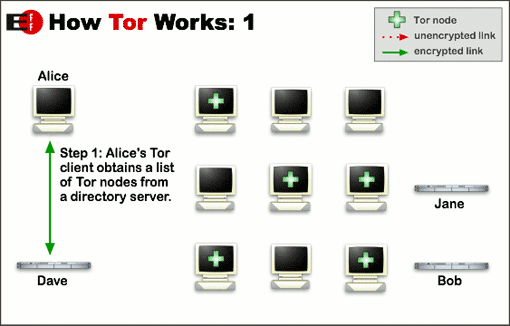
\includegraphics[scale=0.54]{img/tor1.png}
\end{center}
\end{frame}

\begin{frame}{Tor}{Tor workings}
\begin{center}
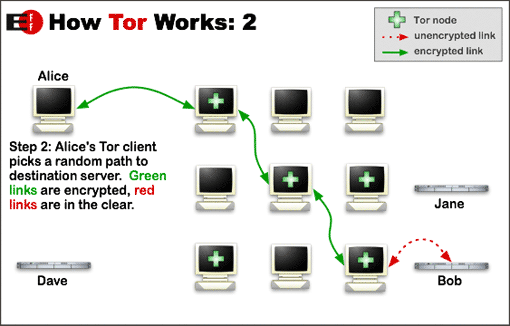
\includegraphics[scale=0.54]{img/tor2.png}
\end{center}
\end{frame}

\begin{frame}{Tor}{Tor workings}
\begin{center}
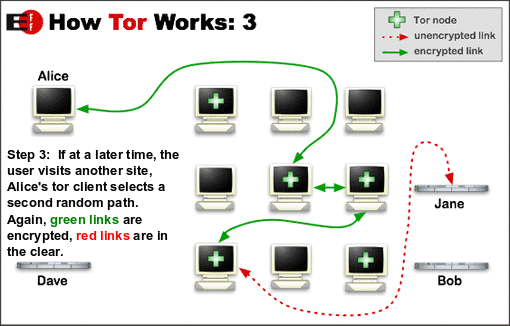
\includegraphics[scale=0.72]{img/tor3.png}
\end{center}
\end{frame}

\begin{frame}{Tor}{Tor encryption}
\begin{center}
	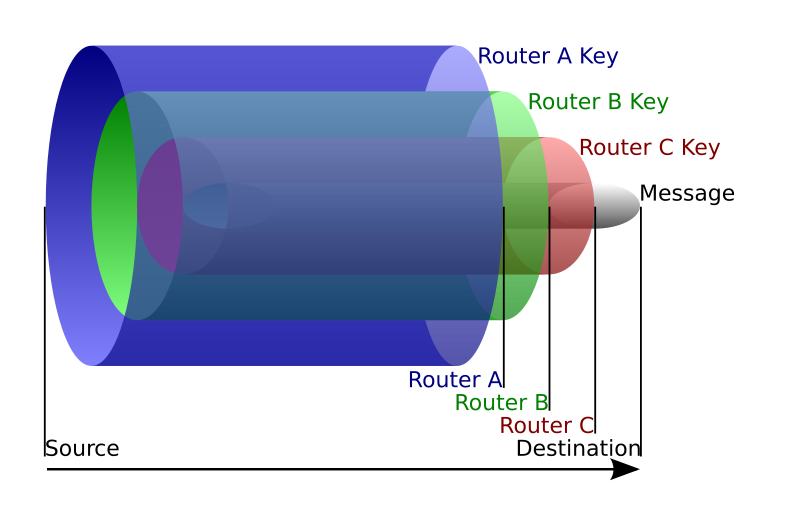
\includegraphics[scale=0.35]{img/onion.png}
\end{center}
\end{frame}

\begin{frame}{Tor}{Tor encryption}
\begin{center}
	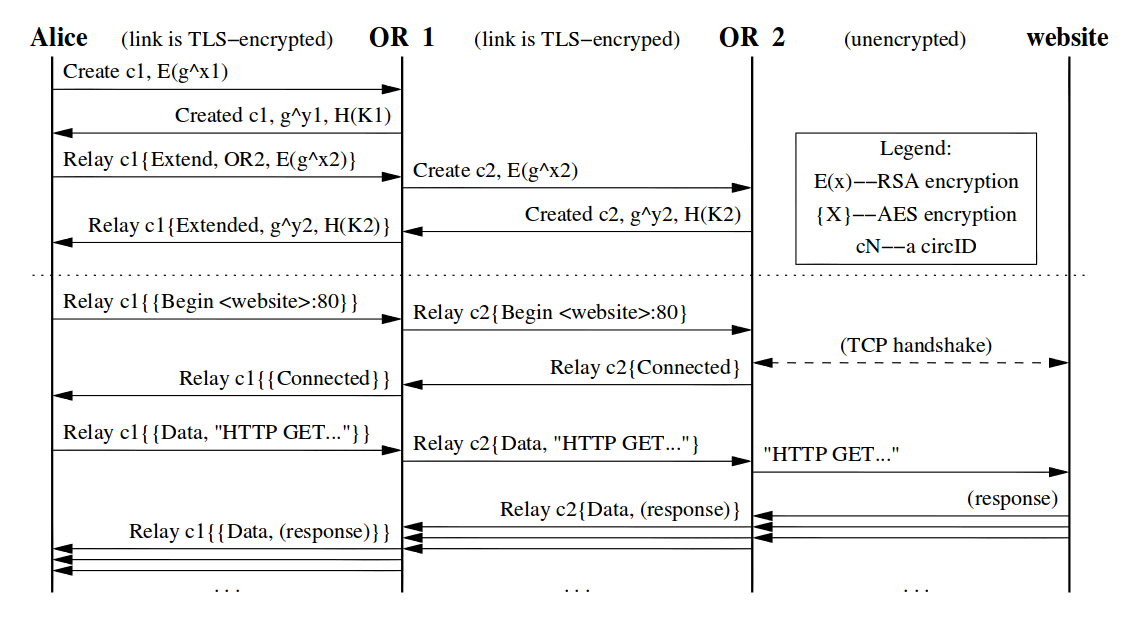
\includegraphics[scale=0.28]{img/or-communication.png}
\end{center}
\end{frame}
\subsection{Attacks}
\begin{frame}{Attacks}{}
	A lot of attacks and vulnerabilities has been discovered for the system.
	\begin{itemize}
		\item Bad apple attack.
		\item Side channel attacks (tor bundle).
		\item Cypher attacks (Tor changed the cryptosystem a lot of time).
		\item \emph{Time analysis based attacks}
		\item Sniper attack.
		\item Sybil attack.
	\end{itemize}
\end{frame}

\begin{frame}{Time analysis based attacks}{}
	\begin{quote}
		\emph{``Tor does not provide protection against end-to-end timing attacks[...]''}
	\end{quote}
	We can place a tracker after the client node and another before the server node
	and check for the connection time to profile users and nodes (and later associate IP to users.)
\end{frame}

\section{Simulation}
\begin{frame}{Simulation}{}
	\begin{itemize}
		\item From this idea we started our simulation work.
		\item But \textbf{OmNet++} doesn't have a reliable simulation
		      model of Tor\footnote{And Tor is fully implemented in
		      User-Space (over level 4)} and so \textbf{NS2/3}.
		\item We needed a simulation model for Tor.
	\end{itemize}
\end{frame}

\subsection{Shadow}
\begin{frame}{Shadow}{Introduction}
	\begin{itemize}
		\item We used the \textbf{Shadow} simulator
		\item Developed by \textbf{Rob Jansen} (U.S. Naval Research Lab).
	\end{itemize}
	\begin{block}{Users}
		
\includegraphics[width=\textwidth]{img/shadow-users.png}
	\end{block}
\end{frame}

\begin{frame}{Shadow}{Simulator internals}
	\begin{minipage}{\textwidth}
	The main feature of \textbf{shadow} is the capability of running real
	applications (like tor).
	\end{minipage}
	\begin{minipage}{0.45\textwidth}
	\small
	Shadow combines virtualization with simulation, it virtualize network
	stacks and act as an micro system hypervisor (partial virtualization).
	\normalsize
	\end{minipage}
	\begin{minipage}{0.4\textwidth}
	\begin{center}
		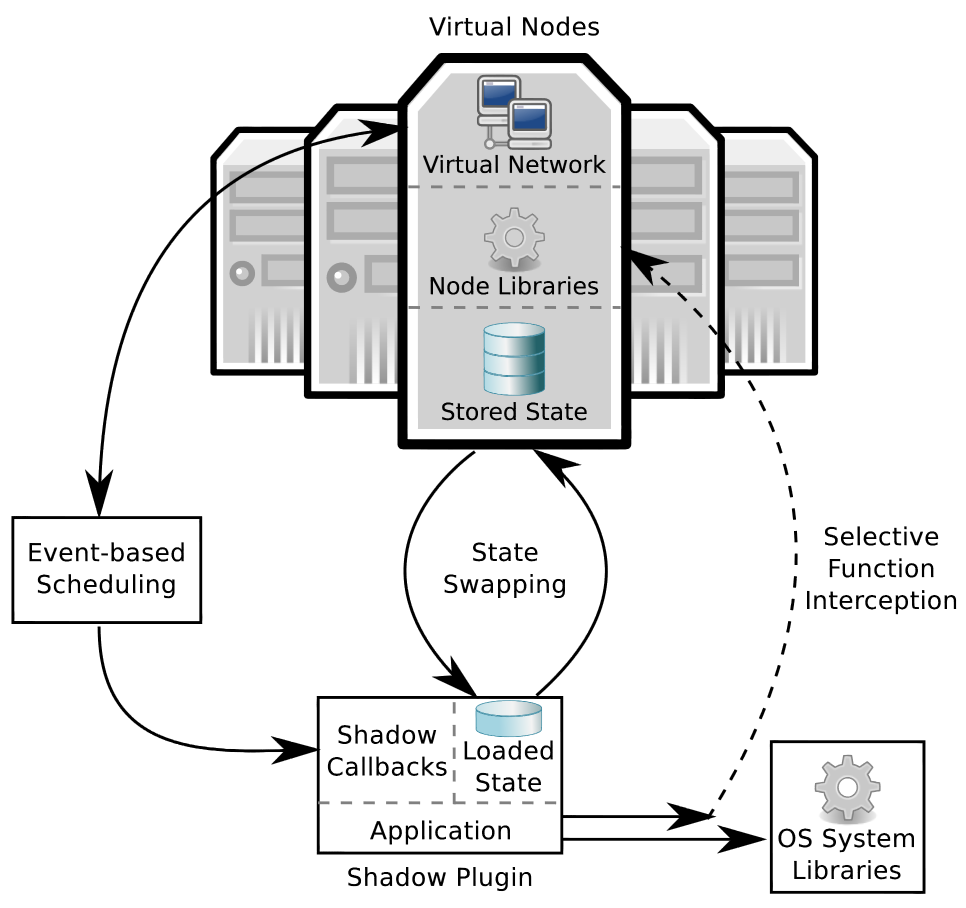
\includegraphics[scale=0.17]{img/shadow.png}
	\end{center}
	\end{minipage}
\end{frame}

\subsection{Plug-ins}

\begin{frame}{Plug-ins}{Shadow plugins}
	So we needed:
	\begin{enumerate}
		\item A client tracer shadow plug-in (proxy).
		\item A server tracer shadow plug-in (proxy).
		\item A logger plug-in.
		\item A client plug-in (HTTP browser?).
		\item A server plug-in (HTTP web-server?).
	\end{enumerate}
	1,2 and 3 was not implemented by the shadow research team.
\end{frame}

\begin{frame}{Plug-ins}{Autosys plug-in}
	\begin{itemize}
		\item Trace the SYN flag that pass trough Tor (on both ways)\footnote{
			        A future work could be the trace of the SYN-ACK flag,
		                to get the corresponding gap in the analysis part.}.
		\item Send a packet to the logger $< type(Tracked\_node) ; Hostname(Tracked\_node) ; timestamp >$.
	\end{itemize}
	\begin{center}
		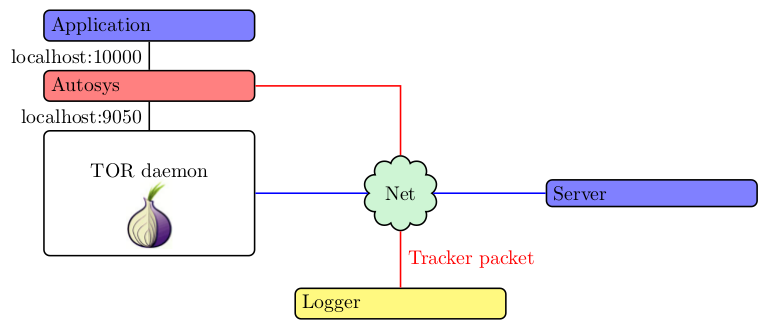
\includegraphics[scale=0.3]{img/autosys.png}
	\end{center}
\end{frame}

\begin{frame}{Plug-ins}{Autosys plug-in}
	Can be implemented in a lot of different ways:
	\begin{itemize}
		\item As a sniffer installed on the routers which listen for
		      every TCP SYN flag (the autonomous system).
		\begin{itemize}
			\item But \textbf{Shadow} does not support Raw Sockets.
		\end{itemize}
		\item We decided to implement that as a simple malware-like connection proxy
		      installed on the client virtual node\footnote{A similar
		      solution to the Hacking team one.}.
		\item Otherwise the tracer can be installed on the guard relay
		      (but we need to deal with re-association between traced
		      clients and real clients because the path changes every
		      10 minutes).
	\end{itemize}
	\begin{center}
		
\includegraphics[scale=0.4]{img/fbi.png}
	\end{center}
\end{frame}

\begin{frame}{Plug-ins}{Analyzer/Logger plug-in}
	\begin{itemize}
		\item After being captured by the sniffers the data must be stocked for late-processing.
		\item We used a public logger service that logs this informations.
		\item Based on UDP for lightness.
		\item (In a real-world scenario this entity would have some form of security and could be replicated/load balanced).
	\end{itemize}
	\begin{center}
		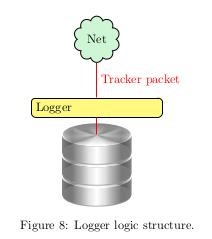
\includegraphics[scale=0.4]{img/logger.png}
	\end{center}
\end{frame}

\begin{frame}{Plug-ins}{Analyzer/Logger plug-in format}
	This plug-in so will save the data that it receives from the sniffers
	with a common format:
	\[ host\_type ; hostname ; timestamp \]
	\begin{itemize}
		\item $host\_type$: C or S if the tracked is a client or a server (the communication is going in or it exiting from Tor?).
		\item $hostname$: The hostname of the tracked (got by autosys).
		\item $timestamp$: The temporal reference of the connection (This will be used to compute distances and gaps).
	\end{itemize}
	This will be processed in the phase 2 to get the matches.
\end{frame}

\begin{frame}{Plug-ins}{SimpleTCP plug-in (Client)}
	We needed a simple client that sends his hostname on the network to compute
	the \textbf{matching accuracy} later.
	\begin{itemize}
		\item Do some connections to a fixed server.
		\item A future work should make it capable of multiple
		      connections to multiple serves.
		\item This plug-in must have SOCKS5 capability to run over Tor.
	\end{itemize}
\end{frame}

\begin{frame}{Plug-ins}{SimpleTCP plug-in (Server)}
	The server part, by opposite:
	\begin{itemize}
		\item Listen for some connections from the clients.
		\item Add a time stamp to the current received packet (correspondent host name).
		\item Save this data to a common file (per server).
	\end{itemize}
	This data will be used in the phase 2 to compute the \textbf{matching accuracy}.
\end{frame}

\begin{frame}{Plug-ins}{The big picture}
	\begin{center}
		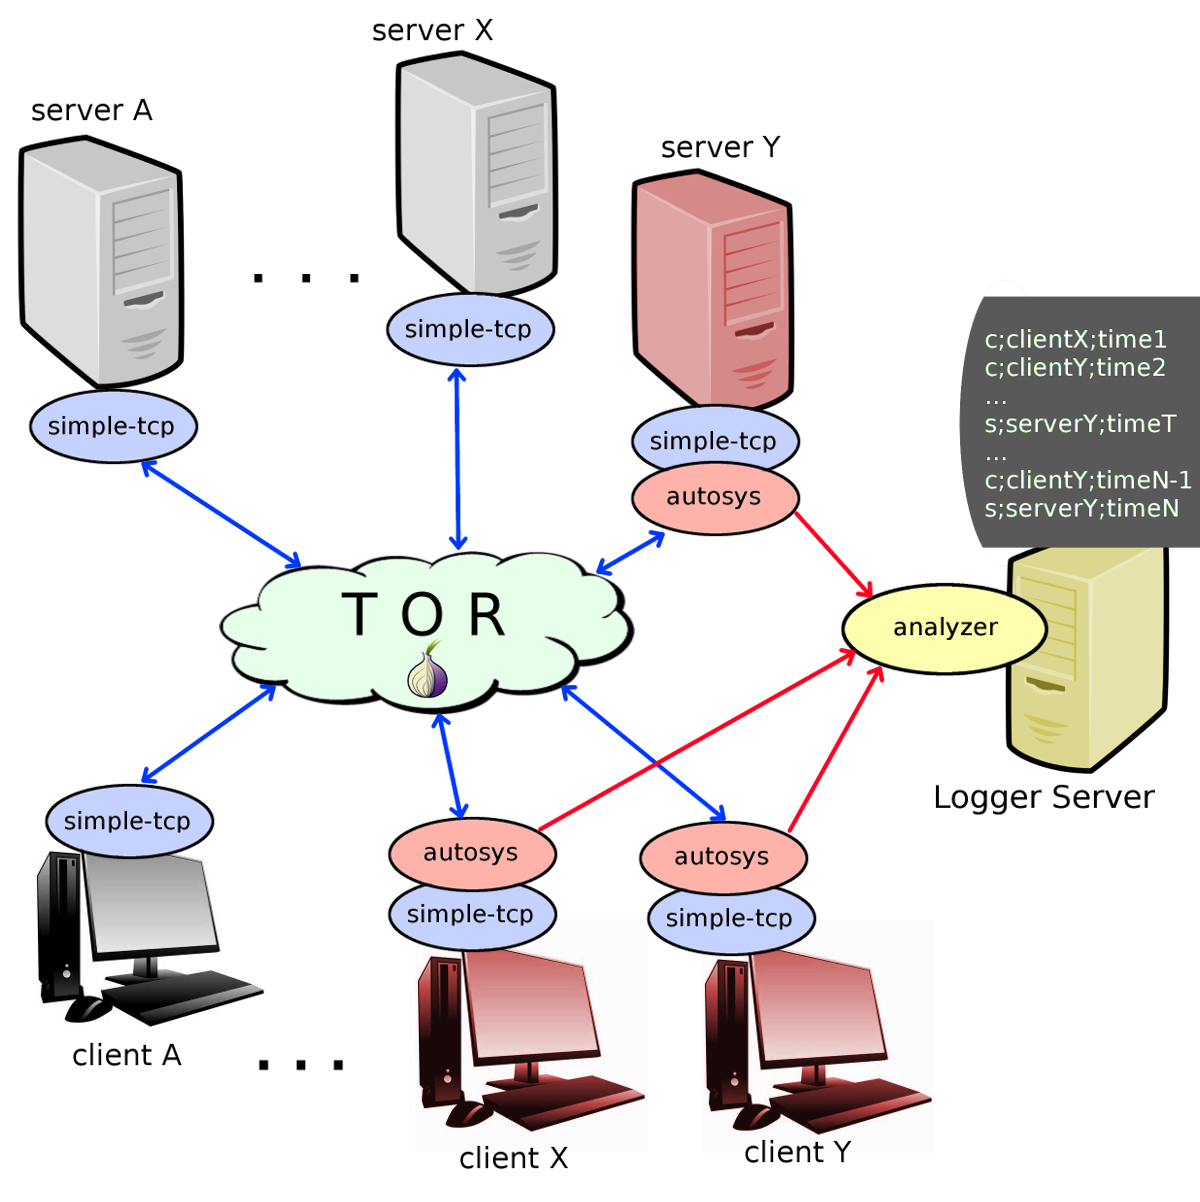
\includegraphics[scale=0.15]{img/scenario.png}
	\end{center}
\end{frame}
